\documentclass[aspectratio=169,10pt]{beamer}

% =========================================================================
% THEME & STYLING CONFIGURATION (NO BLACK BAR ARTIFACTS)
% =========================================================================
\usetheme{Madrid}
\usecolortheme{whale}
\usecolortheme{orchid}

% Disable PDF transparency shadows that previewers render as black bars
\setbeamertemplate{blocks}[rounded][shadow=false]
\setbeamertemplate{title page}[default][colsep=-4bp,rounded=true,shadow=false]
\setbeamertemplate{navigation symbols}{}

% Refined academic color palette
\definecolor{primaryblue}{RGB}{20, 55, 110}
\definecolor{secondaryblue}{RGB}{41, 128, 185}
\definecolor{accentteal}{RGB}{22, 160, 133}
\definecolor{darkgray}{RGB}{44, 62, 80}
\definecolor{lightbg}{RGB}{245, 247, 250}
\definecolor{alertred}{RGB}{192, 57, 43}
\definecolor{examplegreen}{RGB}{39, 174, 96}

\setbeamercolor{palette primary}{bg=primaryblue,fg=white}
\setbeamercolor{palette secondary}{bg=secondaryblue,fg=white}
\setbeamercolor{palette tertiary}{bg=primaryblue,fg=white}
\setbeamercolor{structure}{fg=primaryblue}
\setbeamercolor{titlelike}{parent=palette primary}
\setbeamercolor{block title}{bg=primaryblue,fg=white}
\setbeamercolor{block body}{bg=lightbg,fg=darkgray}
\setbeamercolor{block title example}{bg=examplegreen,fg=white}
\setbeamercolor{block body example}{bg=lightbg,fg=darkgray}
\setbeamercolor{block title alerted}{bg=alertred,fg=white}
\setbeamercolor{block body alerted}{bg=lightbg,fg=darkgray}

% Custom clean footline
\setbeamertemplate{footline}{
  \leavevmode%
  \hbox{%
  \begin{beamercolorbox}[wd=.333333\paperwidth,ht=2.25ex,dp=1ex,center]{author in head/foot}%
    \usebeamerfont{author in head/foot}\insertshortauthor
  \end{beamercolorbox}%
  \begin{beamercolorbox}[wd=.333333\paperwidth,ht=2.25ex,dp=1ex,center]{title in head/foot}%
    \usebeamerfont{title in head/foot}\insertshorttitle
  \end{beamercolorbox}%
  \begin{beamercolorbox}[wd=.333333\paperwidth,ht=2.25ex,dp=1ex,right]{date in head/foot}%
    \usebeamerfont{date in head/foot}\insertshortdate{}\hspace*{2em}
    \insertframenumber{} / \inserttotalframenumber\hspace*{2ex} 
  \end{beamercolorbox}}%
  \vskip0pt%
}

% =========================================================================
% PACKAGES
% =========================================================================
\usepackage{amsmath,amssymb,amsfonts,mathtools}
\usepackage{graphicx}
\usepackage{booktabs}
\usepackage{tikz}
\usepackage{pgfplots}
\pgfplotsset{compat=1.18}

% =========================================================================
% TITLE & METADATA
% =========================================================================
\title[Calculus for Computing]{Functions of Several Variables}
\subtitle{Chapter 4 (Part 1): Functions of More than One Variable, Domains \& Level Curves}
\author[Faculty of IT, TDTU]{Department of Mathematics \& Computer Science}
\institute[TDTU]{Applied Calculus for IT 2 (Course Code: 501033) -- Ton Duc Thang University}
\date{\today}

% =========================================================================
% DOCUMENT BODY
% =========================================================================
\begin{document}

% -------------------------------------------------------------------------
% Title Slide
% -------------------------------------------------------------------------
\begin{frame}[plain]
  \titlepage
\end{frame}

% -------------------------------------------------------------------------
% Table of Contents
% -------------------------------------------------------------------------
\begin{frame}{Table of Contents}
  \tableofcontents
\end{frame}

% =========================================================================
% SECTION 1: FUNCTIONS OF MORE THAN ONE VARIABLE & DOMAINS
% =========================================================================
\section{Functions of More than One Variable}

\begin{frame}{Motivation: Quantities with Multiple Inputs (Slide 3)}
  In real-world applications, many objects and quantities are determined by \textbf{more than one independent variable}:

  \vspace{0.2em}
  \begin{columns}[T]
    \begin{column}{0.48\textwidth}
      \begin{block}{Geometric Examples}
        \small
        \begin{itemize}
          \item \textbf{Area of a rectangle}:
          \[
            A = xy
          \]
          ($x$ is length, $y$ is width).
          
          \vspace{0.1em}
          \item \textbf{Volume of a circular cone}:
          \[
            V = \frac{1}{3}\pi r^2 h
          \]
          ($r$ is radius, $h$ is height).
        \end{itemize}
      \end{block}
    \end{column}

    \begin{column}{0.48\textwidth}
      \begin{block}{Physical Examples}
        \small
        \begin{itemize}
          \item \textbf{Kinetic energy}:
          \[
            E_k = \frac{1}{2}m v^2
          \]
          ($m$ is mass, $v$ is velocity).

          \vspace{0.1em}
          \item \textbf{Potential energy}:
          \[
            E_p = mgh
          \]
          ($m$ is mass, $h$ is height).
        \end{itemize}
      \end{block}
    \end{column}
  \end{columns}
\end{frame}

\begin{frame}{Functions of Two Variables \& Natural Domain (Slide 4)}
  \begin{definition}[Function of Two Variables]
    Let $z = f(x, y)$ be a function with two variables $x$ and $y$.
    \begin{itemize}
      \item $x$ and $y$ are the \textbf{independent variables}.
      \item $z$ is the \textbf{dependent variable}.
      \item Unless otherwise specified, the \textbf{domain} $D$ is the \textbf{largest subset of $\mathbb{R}^2$} on which $f$ is mathematically well-defined.
    \end{itemize}
  \end{definition}

  \vspace{0.2em}
  \begin{block}{Boundary Convention for Domains in $\mathbb{R}^2$}
    \small
    \begin{itemize}
      \item \textbf{Strict inequality ($>$ or $<$)}: Boundary drawn as a \textbf{dashed curve} (points excluded).
      \item \textbf{Non-strict inequality ($\ge$ or $\le$)}: Boundary drawn as a \textbf{solid curve} (points included).
    \end{itemize}
  \end{block}
\end{frame}

\begin{frame}{Domain Example 1: Parabola and Line Restrictions (Slide 4)}
  \begin{exampleblock}{Example (MA1521 Slide 4)}
    Find and sketch the domain of $f(x, y) = \dfrac{x + 2y}{\sqrt{x - y^2}} + \ln(8 - x - y)$.
  \end{exampleblock}

  \begin{columns}[T]
    \begin{column}{0.55\textwidth}
      \begin{block}{Algebraic Conditions}
        \footnotesize
        We have two simultaneous conditions:
        \begin{enumerate}
          \item $\dfrac{1}{\sqrt{x - y^2}}: \quad x - y^2 > 0 \iff x > y^2$\\
          \textit{(Region strictly to the right of parabola $x = y^2$)}
          \item $\ln(8 - x - y): \quad 8 - x - y > 0 \iff x + y < 8$\\
          \textit{(Region strictly below line $x + y = 8$)}
        \end{enumerate}
        \textbf{Domain Set}:
        \[
          D = \{(x, y) \in \mathbb{R}^2 \mid x > y^2 \text{ and } x + y < 8\}.
        \]
      \end{block}
    \end{column}

    \begin{column}{0.42\textwidth}
      \centering
      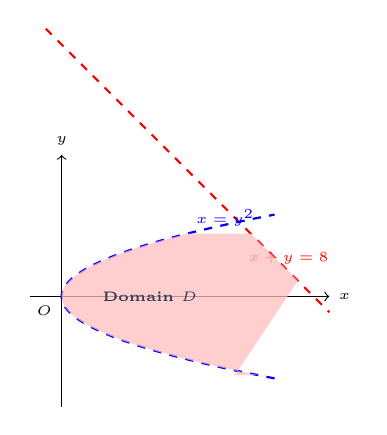
\begin{tikzpicture}[scale=0.40]
        \draw[->] (-1,0) -- (8.5,0) node[right] {\tiny $x$};
        \draw[->] (0,-3.5) -- (0,4.5) node[above] {\tiny $y$};
        \node[below left] at (0,0) {\tiny $O$};

        % Line x + y = 8 (dashed)
        \draw[dashed, red, thick] (-0.5, 8.5) -- (8.5, -0.5);
        \node[red] at (7.2, 1.2) {\tiny $x+y=8$};

        % Parabola x = y^2 (dashed)
        \draw[dashed, blue, thick, domain=-2.6:2.6, samples=40] plot ({\x*\x}, \x);
        \node[blue] at (5.2, 2.5) {\tiny $x=y^2$};

        % Shaded intersection area
        \fill[red!25, opacity=0.75, domain=-2.5:2.0, samples=40] 
          plot ({\x*\x}, \x) -- (6.0, 2.0) -- (7.5,0.5) -- (5.5,-2.5) -- cycle;
        
        \node[darkgray] at (2.8, 0) {\tiny \textbf{Domain $D$}};
      \end{tikzpicture}
    \end{column}
  \end{columns}
\end{frame}

\begin{frame}{Domain Example 2: Linear Inequality (Slide 5)}
  \begin{exampleblock}{Example (MA1521 Slide 5)}
    Find and sketch the domain of $f(x, y) = \ln(10 - 2x - 3y)$.
  \end{exampleblock}

  \begin{columns}[T]
    \begin{column}{0.55\textwidth}
      \begin{block}{Algebraic Condition}
        \small
        The natural logarithm requires a strictly positive argument:
        \[
          \ln(10 - 2x - 3y): \quad 10 - 2x - 3y > 0 \iff 2x + 3y < 10.
        \]
        \begin{itemize}
          \item \textbf{Boundary line}: $2x + 3y = 10$ ($x$-intercept $5$, $y$-intercept $10/3$).
          \item Inequality is strict ($<$): Boundary is drawn as a \textbf{dashed line}.
          \item Testing $(0,0)$: $0 < 10$ (True $\implies$ side containing origin).
        \end{itemize}
        \textbf{Domain Set}: $D = \left\{(x, y) \in \mathbb{R}^2 \mid 2x + 3y < 10 \right\}$.
      \end{block}
    \end{column}

    \begin{column}{0.42\textwidth}
      \centering
      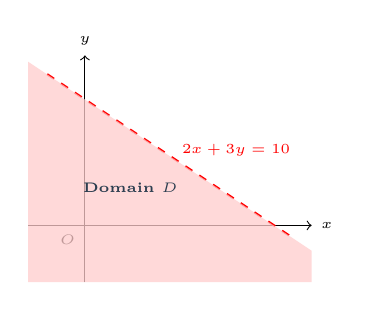
\begin{tikzpicture}[scale=0.48]
        \draw[->] (-1.5,0) -- (6,0) node[right] {\tiny $x$};
        \draw[->] (0,-1.5) -- (0,4.5) node[above] {\tiny $y$};
        \node[below left] at (0,0) {\tiny $O$};

        % Boundary line 2x + 3y = 10
        \draw[dashed, red, thick] (-1, 4) -- (5.5, -0.33);
        \node[red] at (4.0, 2.0) {\tiny $2x+3y=10$};

        % Shaded half-plane
        \fill[red!20, opacity=0.75] (-1.5,-1.5) -- (6,-1.5) -- (6,-0.67) -- (-1.5, 4.33) -- cycle;
        \node[darkgray] at (1.2, 1.0) {\tiny \textbf{Domain $D$}};
      \end{tikzpicture}
    \end{column}
  \end{columns}
\end{frame}

\begin{frame}{Domain Example 3: Function of Three Variables (Slide 5)}
  \begin{exampleblock}{Example (MA1521 Slide 5)}
    Find and describe the domain of $f(x, y, z) = \sqrt{9 - (x^2 + y^2 + z^2)}$.
  \end{exampleblock}

  \begin{columns}[T]
    \begin{column}{0.55\textwidth}
      \begin{block}{Algebraic Condition in $\mathbb{R}^3$}
        \small
        The radicand of the square root must be non-negative:
        \[
          9 - (x^2 + y^2 + z^2) \ge 0 \iff x^2 + y^2 + z^2 \le 9 = 3^2.
        \]
        \begin{itemize}
          \item Boundary is the sphere $x^2 + y^2 + z^2 = 9$ of radius $R = 3$ centered at origin $O(0,0,0)$.
          \item The inequality ($\le$) includes the boundary sphere.
        \end{itemize}
        \textbf{Conclusion}: Domain $D$ is the \textbf{solid ball} of center $O$ and radius $3$.
      \end{block}
    \end{column}

    \begin{column}{0.42\textwidth}
      \centering
      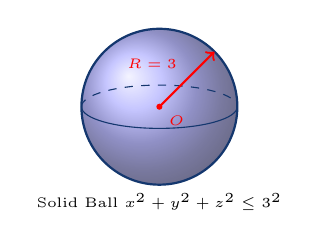
\begin{tikzpicture}[scale=0.55]
        \shade[ball color = blue!40, opacity = 0.75] (0,0) circle (1.8);
        \draw[thick, primaryblue] (0,0) circle (1.8);
        \draw[dashed, primaryblue] (-1.8,0) arc (180:0:1.8 and 0.5);
        \draw[primaryblue] (-1.8,0) arc (180:360:1.8 and 0.5);
        \fill[red] (0,0) circle (2pt) node[below right] {\tiny $O$};
        \draw[->, thick, red] (0,0) -- (1.27, 1.27) node[midway, above left] {\tiny $R=3$};
        \node at (0, -2.2) {\tiny Solid Ball $x^2+y^2+z^2 \le 3^2$};
      \end{tikzpicture}
    \end{column}
  \end{columns}
\end{frame}

% =========================================================================
% SECTION 2: GRAPH OF TWO-VARIABLE FUNCTION & LEVEL CURVES
% =========================================================================
\section{Graph of Two-Variable Function \& Level Curves}

\begin{frame}{Graph of a Two-Variable Function (Slide 6)}
  \begin{definition}[Graph in $\mathbb{R}^3$]
    The \textbf{graph} of function $z = f(x, y)$ with domain $D$ is:
    \[
      \{(x, y, z) \in \mathbb{R}^3 \mid (x, y) \in D \text{ and } z = f(x, y)\}.
    \]
    It is a \textbf{surface} defined by the function.
  \end{definition}

  \begin{block}{Question: How can we plot a surface?}
    \small
    \begin{itemize}
      \item For $s = g(t)$, we pick points $t_1, \dots, t_n$ and connect points with a smooth curve.
      \item For $z = f(x, y)$, this method fails. Instead:
      \begin{itemize}
        \item For each $z = z_0$, draw the \textbf{level curve} $z_0 = f(x, y)$.
        \item This is the \textbf{intersection} of the surface $z = f(x, y)$ and the horizontal plane $z = z_0$:
        \[
          L_{z_0} := \{(x, y) \mid f(x, y) = z_0\}.
        \]
      \end{itemize}
    \end{itemize}
  \end{block}
\end{frame}

\begin{frame}{Level Curves Example 1: Linear Surface (Slide 7)}
  \begin{exampleblock}{Example (MA1521 Slide 7)}
    Draw the level curves of $f(x, y) = 10 - 2x - y$.
  \end{exampleblock}

  \begin{columns}[T]
    \begin{column}{0.5\textwidth}
      \begin{block}{Family of Level Curves}
        \small
        Set $f(x, y) = k$:
        \[
          10 - 2x - y = k \iff 2x + y = 10 - k.
        \]
        \begin{itemize}
          \item For each $k$, this is a straight line with slope $m = -2$.
          \item For $k = -5, -4, -3, -2, -1, 0, 1, 2, 3, 4$:
          \item The level curves form a family of \textbf{parallel straight lines}.
          \item The 3D surface $z = 10 - 2x - y$ is a \textbf{plane}.
        \end{itemize}
      \end{block}
    \end{column}

    \begin{column}{0.48\textwidth}
      \centering
      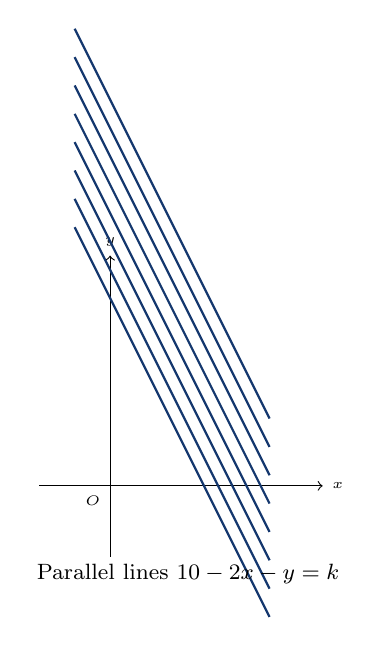
\begin{tikzpicture}[scale=0.45]
        \draw[->] (-2,0) -- (6,0) node[right] {\tiny $x$};
        \draw[->] (0,-2) -- (0,6.5) node[above] {\tiny $y$};
        \node[below left] at (0,0) {\tiny $O$};

        \foreach \k in {-3, -2, -1, 0, 1, 2, 3, 4} {
          \draw[primaryblue, thick] (-1, {8.5 - \k*0.8 + 2}) -- (4.5, {8.5 - \k*0.8 - 9});
        }
        \node at (2.2, -2.5) {\footnotesize Parallel lines $10-2x-y=k$};
      \end{tikzpicture}
    \end{column}
  \end{columns}
\end{frame}

\begin{frame}{Level Curves Example 2: Circular Paraboloid (Slide 8)}
  \begin{exampleblock}{Example (MA1521 Slide 8)}
    Draw the level curves of $f(x, y) = x^2 + y^2$.
  \end{exampleblock}

  \begin{columns}[T]
    \begin{column}{0.5\textwidth}
      \begin{block}{Family of Level Curves}
        \small
        Set $f(x, y) = k$ ($k \ge 0$):
        \[
          x^2 + y^2 = k.
        \]
        \begin{itemize}
          \item $k = 0$: Single point $(0, 0)$ at apex/vertex.
          \item $k = 1, 2, 3, 4, 5, 6, 7, 8, 9$:
          \item Concentric circles of radii $r = \sqrt{k}$.
          \item Circles become \textbf{closer together} as $k$ grows $\implies$ surface becomes \textbf{steeper}.
          \item The 3D surface is a \textbf{Circular Paraboloid}.
        \end{itemize}
      \end{block}
    \end{column}

    \begin{column}{0.48\textwidth}
      \centering
      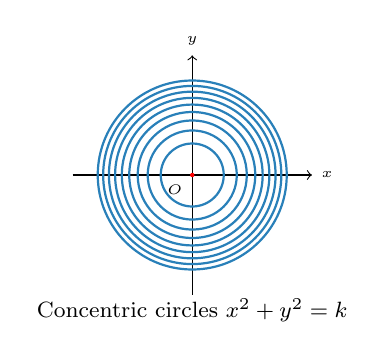
\begin{tikzpicture}[scale=0.40]
        \draw[->] (-3.8,0) -- (3.8,0) node[right] {\tiny $x$};
        \draw[->] (0,-3.8) -- (0,3.8) node[above] {\tiny $y$};
        \node[below left] at (0,0) {\tiny $O$};

        \fill[red] (0,0) circle (2pt);
        \foreach \k in {1, 2, 3, 4, 5, 6, 7, 8, 9} {
          \draw[secondaryblue, thick] (0,0) circle ({sqrt(\k)*1.0});
        }
        \node at (0, -4.3) {\footnotesize Concentric circles $x^2+y^2=k$};
      \end{tikzpicture}
    \end{column}
  \end{columns}
\end{frame}

\begin{frame}{Level Curves Example 3: Circular Cone (Slide 9)}
  \begin{exampleblock}{Example (MA1521 Slide 9)}
    Draw the level curves of $f(x, y) = \sqrt{x^2 + y^2}$.
  \end{exampleblock}

  \begin{columns}[T]
    \begin{column}{0.5\textwidth}
      \begin{block}{Family of Level Curves}
        \small
        Set $f(x, y) = k$ ($k \ge 0$):
        \[
          \sqrt{x^2 + y^2} = k \iff x^2 + y^2 = k^2.
        \]
        \begin{itemize}
          \item $k = 0$: Single point $(0, 0)$.
          \item $k = 1, 2, 3, 4, 5, 6, 7, 8, 9$:
          \item Circles centered at origin with radii $r = k$.
          \item Circles are \textbf{equally spaced} ($\Delta r = 1$) $\implies$ surface has \textbf{constant slope}.
          \item The 3D surface is a \textbf{Circular Cone}.
        \end{itemize}
      \end{block}
    \end{column}

    \begin{column}{0.48\textwidth}
      \centering
      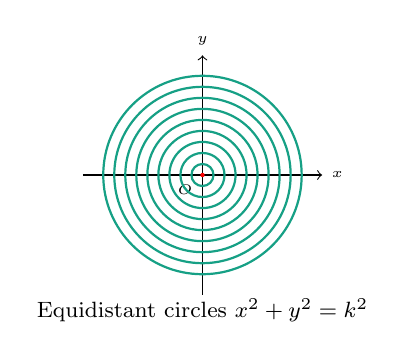
\begin{tikzpicture}[scale=0.40]
        \draw[->] (-3.8,0) -- (3.8,0) node[right] {\tiny $x$};
        \draw[->] (0,-3.8) -- (0,3.8) node[above] {\tiny $y$};
        \node[below left] at (0,0) {\tiny $O$};

        \fill[red] (0,0) circle (2pt);
        \foreach \k in {1, 2, 3, 4, 5, 6, 7, 8, 9} {
          \draw[accentteal, thick] (0,0) circle ({\k * 0.35});
        }
        \node at (0, -4.3) {\footnotesize Equidistant circles $x^2+y^2=k^2$};
      \end{tikzpicture}
    \end{column}
  \end{columns}
\end{frame}

\begin{frame}{Level Curves Example 4: Hyperbolic Paraboloid (Slide 10)}
  \begin{exampleblock}{Example (MA1521 Slide 10)}
    Draw the level curves of $f(x, y) = x^2 - y^2$.
  \end{exampleblock}

  \begin{columns}[T]
    \begin{column}{0.5\textwidth}
      \begin{block}{Family of Level Curves}
        \small
        Set $f(x, y) = k$:
        \[
          x^2 - y^2 = k.
        \]
        \begin{itemize}
          \item $k = 0$: Pair of intersecting lines $y = \pm x$.
          \item $k > 0$: Hyperbolas opening along the $x$-axis.
          \item $k < 0$: Hyperbolas opening along the $y$-axis.
          \item The 3D surface is a \textbf{Hyperbolic Paraboloid (Saddle Surface)}.
          \item Origin $(0, 0)$ is a \textbf{saddle point}.
        \end{itemize}
      \end{block}
    \end{column}

    \begin{column}{0.48\textwidth}
      \centering
      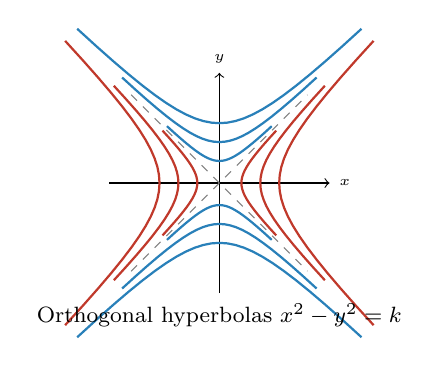
\begin{tikzpicture}[scale=0.40]
        \draw[->] (-3.5,0) -- (3.5,0) node[right] {\tiny $x$};
        \draw[->] (0,-3.5) -- (0,3.5) node[above] {\tiny $y$};

        % Asymptotes k = 0
        \draw[dashed, gray] (-2.8,-2.8) -- (2.8,2.8);
        \draw[dashed, gray] (-2.8,2.8) -- (2.8,-2.8);

        % Hyperbolas k > 0
        \foreach \a in {0.7, 1.3, 1.9} {
          \draw[alertred, thick, domain=-1.6:1.6] plot ({\a*cosh(\x)}, {\a*sinh(\x)});
          \draw[alertred, thick, domain=-1.6:1.6] plot ({-\a*cosh(\x)}, {\a*sinh(\x)});
        }
        % Hyperbolas k < 0
        \foreach \a in {0.7, 1.3, 1.9} {
          \draw[secondaryblue, thick, domain=-1.6:1.6] plot ({\a*sinh(\x)}, {\a*cosh(\x)});
          \draw[secondaryblue, thick, domain=-1.6:1.6] plot ({\a*sinh(\x)}, {-\a*cosh(\x)});
        }
        \node at (0, -4.2) {\footnotesize Orthogonal hyperbolas $x^2-y^2=k$};
      \end{tikzpicture}
    \end{column}
  \end{columns}
\end{frame}

% =========================================================================
% SECTION 3: SUMMARY & KEY TAKEAWAYS
% =========================================================================
\section{Summary \& Key Takeaways}

\begin{frame}{Summary Checklist: Functions of Several Variables}
  \begin{columns}[T]
    \begin{column}{0.48\textwidth}
      \begin{block}{Part 1: Functions \& Domains}
        \small
        \begin{itemize}
          \item \textbf{Function $z = f(x, y)$}: Independent variables $x, y \in D \subset \mathbb{R}^2$, dependent variable $z \in \mathbb{R}$.
          \item \textbf{Natural Domain}: Largest subset of $\mathbb{R}^2$ (or $\mathbb{R}^n$) where $f$ is well-defined.
          \item \textbf{Algebraic Rules}: Fractions $Q \neq 0$, Radicals $\sqrt{g} \ge 0$, Logs $\ln(g) > 0$.
          \item \textbf{Boundaries}: $\ge, \le \implies$ solid; $>, < \implies$ dashed.
        \end{itemize}
      \end{block}
    \end{column}

    \begin{column}{0.48\textwidth}
      \begin{block}{Part 2: Graphs \& Level Curves}
        \small
        \begin{itemize}
          \item \textbf{Graph}: 3D surface $z = f(x, y)$ in $\mathbb{R}^3$.
          \item \textbf{Level Curves}: $L_{z_0} = \{(x, y) \mid f(x, y) = z_0\}$.
          \item \textbf{Plane}: $10-2x-y = k \implies$ parallel lines.
          \item \textbf{Paraboloid}: $x^2+y^2 = k \implies$ circles ($r=\sqrt{k}$).
          \item \textbf{Cone}: $\sqrt{x^2+y^2} = k \implies$ circles ($r=k$).
          \item \textbf{Saddle}: $x^2-y^2 = k \implies$ hyperbolas.
        \end{itemize}
      \end{block}
    \end{column}
  \end{columns}

  \vspace{0.6em}
  \centering
  \textbf{Next Topic (Slide 11)}: \textit{Partial Derivatives $\dfrac{\partial z}{\partial x}, \dfrac{\partial z}{\partial y}$ and Gradient Vector $\nabla f$!}
\end{frame}

% -------------------------------------------------------------------------
% Final Q&A Slide
% -------------------------------------------------------------------------
\begin{frame}[plain]
  \begin{center}
    \vspace{2cm}
    {\Huge \bfseries \color{primaryblue} Thank You!}\\[1em]
    {\large Questions \& Discussion}\\[1.5em]
    \textit{Chapter 4 (Part 1): Functions of More than One Variable}
  \end{center}
\end{frame}

\end{document}
